\documentclass[11pt, letterpaper]{article}

% -------------------------------------------------------------------------
% Commands
\usepackage[utf8]{inputenc}
\usepackage{graphicx}
\usepackage{hyperref}
\usepackage{cite}
\usepackage{vmargin}

\setmargins{2.5cm}                 % margen izquierdo
{1.5cm}                            % margen superior
{16.5cm}                           % anchura del texto
{23.42cm}                          % altura del texto
{10pt}                             % altura de los encabezados
{1cm}                              % espacio entre el texto y los encabezados
{0pt}                              % altura del pie de página
{2cm}                              % espacio entre el texto y el pie de página

% \hyphenation{}

% \hypersetup{colorlinks,%
% 	citecolor=blue,%s
% 	filecolor=blue,%
% 	linkcolor=blue,%
% 	urlcolor=blue%
% }


% -------------------------------------------------------------------------
\title{\textbf{Extending a shadow price-based definition of nutrient limitation to genome-scaled metabolic netwotks in complex mediums}}

% -------------------------------------------------------------------------

\date{}
\author{
  \textbf{Jos\'e A. Pereiro-Morej\'on$^{1,3}$, Roberto Mulet$^{1,2}$} \\
  \small{1. Group of Complex Systems and Statistical Physics.} \\
  \small{Physics Faculty, University of Havana, CP 10400. La Habana, Cuba} \\
  \small{2. Department of Theoretical Physics, }\\
  \small{Physics Faculty Faculty, University of Havana, CP 10400. La Habana, Cuba} \\
  \small{3. Biology Faculty, University of Havana, CP 10400. La Habana, Cuba} \\
}

% -------------------------------------------------------------------------
% opening
\begin{document}

\maketitle

\begin{abstract}
	Nutrient limitation is a culture condition that experimentalists can easily identify, particularly in continuous culture steady states, where the biomass may stabilize due to depletion of a critical nutrient supply. However, reproducing this property in genome-scaled metabolic models is difficult, as its emergent nature lacks a clear mechanism of how such a condition can arise from the state distribution of cells in the culture. In this work, we use a particular, well-defined single-cell definition of nutrient limitation based on the shadow price of the boundary constraints over biomass production. This definition has been proven to work with networks constrained by simple medium compositions and is well supported by experimental data. We aim to extend this procedure to networks constrained by complex mediums, which is the case of mammalian cells cultures. Our results show that we can easily find minimal contraint modifications that produce nutrient-limited subnetworks. In particular, for HEK and CHO networks, there are only a few such minimal sets. This procedure can be used to contextualize metabolic networks to include the nutrient limitation phenotype before further analysis.
\end{abstract}

% We discuss experimental data that supports this definition and propose a simple algorithm for generating nutrient-limited GEMs. We benchmark these GEMs using experimentally-available metabolic fluxes for CHO cultures.

% -------------------------------------------------------------------------
% \section{Dev}

% \subsection{Layout}


% ii. The complexity of the medium, impacts the ammound of information that is required to input into models in order to reproduce the limiting nutrient condictions. 

% - This problem is similar to model the Warburng effect

% iii. Must GEMs do not constraint such information and are unable to handle complex mediums. 

% vi. Single cell definition of nutrient limitation (shadow price)

% iv. The case of E coli cultures (simple medium)

% v. The case of  mammalian cultures (complex medium)

% vi. Compare with data from hazelwoodIdentityGrowthLimitingNutrient2009

% - Yeast transcriptomic data in C and N limited conditions. Compare the transcriptomic pattern with the NL-Networks

% TO_CHECK [10.1016/j.biotechadv.2003.08.006] The "law of the minimum" (Liebig's law) states that usually one nutrient restricts the maximum quantity of biomass that can be produced within a system, whereas all other nutrients are in excess. 


% -------------------------------------------------------------------------
% \section{Introduction}

% Nutrient limitation is a common culture condition that experimentalists can easily identify.
% It is brodly defined as the dependency of the growth parameters of the culture on the availability of a given nutrient.
% In the context of chemostat cultures, this condition often signal the attainment of steady state, as the biomass stabilize due to depletion of the supply of a critical nutrient \cite{
% 	herbertContinuousCultureBacteria1956, 
% 	vriezenEffectsGlutamineSupply1997, % Checked 
% 	natarajanTranscriptionalProfilingShows2001, 
% 	wuGlobalAnalysisNutrient2004, % Checked 
% 	daran-lapujadeRoleTranscriptionalRegulation2004, % Checked 
% 	taiTwodimensionalTranscriptomeAnalysis2005, % Checked 
% 	daran-lapujadeChemostatBasedMicroArrayAnalysis2008, 
% 	hazelwoodIdentityGrowthLimitingNutrient2009, 
% 	boerGrowthlimitingIntracellularMetabolites2010, 
% 	folsomPhysiologicalProteomicAnalysis2014, % Checked 
% 	pereiro-morejonInferenceMetabolicFluxes2022, % Checked ;)
% }.
% Moreover, for economic reasons, industrial applications often employ growth media that are optimized to obtain minimal residual concentrations of expensive nutrients [citation needed].

% In recent years, it has become increasingly common to utilize genome-scale metabolic networks in culture modeling.
% These models have the potential to improve production parameters in industrial processes [citation needed].
% However, it is noteworthy that nutrient limitation, an important phenotype that the models should reproduce, is often overlooked [citation needed].
% The main reason for this gap is the inherent complexity involved in modeling such conditions, which can stem from a variety of factors, ranging from intricate regulatory influences to more evident essential requirements.

% For instance, in a culture where the medium comprises a single carbon source, it is intuitive that if the nutrient is restricted sufficiently, its availability will become a primary factor governing the performance of the culture. Such situations are commonplace in bacterial cultures, where the medium can be very simple [citation needed]. In such cases, models tend to reproduce the limiting condition effortlessly [citation needed].

% Conversely, if the medium is complex and contains several analogous nutrients (such as different carbon sources), the models must be capable of distinguishing between them. However, as we will discuss later, many models are unable to make such distinctions and fail to reproduce the limiting condition. This is often the case for mammalian cell cultures, where even the simplest medium provides multiple carbon and nitrogen sources [citation needed].

% In this work we propose a methodology for modifying genome scale metabolic models to enfore the limiting condition when no further biological data is available. This will allow us to obtain a set of nutrient-limited network that we can explore. 
% % We will explore the space of nutrient-limited network and use some static measurements, .


% % NOTE: Nutrinet limited definition: 
% % We can have many different definitions of nutrient limitation. 
% % In egliConceptMultiplenutrientlimitedGrowth2003 they used the criterio of nutrinet depletion (more generaly yield).
% % In there case the have dual nutrient limitation if there are multiple depleted nutrients.


% % -------------------------------------------------------------------------
% \section{Methodology}

% \subsection{Single cell considerations}

% Modeling nutrient limited cultures is a challenging task because nutrient limitation is an emergent property that results from underlying single-cell processes.
% These processes are known to be heterogeneous, and the information required to comprehensively model them is largely unavailable \cite{palssonSystemBiologyConstraintbased2015}.
% In order to overcome such limitations we make several simplifications.

% A first common simplification is to assume that all cells are described by the same set of constraints.
% These constraints are derived from the definition of the metabolic network and the experimental conditions of the culture.

% The second one deals with the "microscopic" (single cell) definition of nutrinet limitation.
% We consider a metabolic network as being limited with respect to boundary metabolite $i$ if, upon evaluation of a given metabolic objective function, its shadow price $p_i$ is the largest (with the appropiate sign) among all boundary metabolites in the given context.
% In the results discussion, we will discuse how this definition fit experimental data for bacteria cultures.

% \subsection{Network modifications}

% Nutrient limitation can be imposed on a metabolic network through various conceivable mechanisms.
% One way is by adding a cost constraint, which modulates the overall flux distribution [citation needed].
% Such a constraint might account for biologically informed criteria, such as cellular economy, where the cell employ the most efficient available route for the usage of a key metabolite.
% Another way is by modifying the allowable range of the flux values.
% This approach might try to account for regulatory modulation of the activity or availability of enzymes.
% In its extreme case, where a reaction range is set to [0,0] or close enough, it is equivalent to changing the topology of the network by removing reactions.
% Finally, adding reactions is not typically worth considering because a genome-scale metabolic network is expected to contain the totality of reactions described by the genome of the given organism [cite required].

% In this work, we will focus only on the case of topology modification.
% This is mainly due to modeling convenience, and we encourage exploring other strategies.

% \subsection{Exploration scheme}

% For a metabolic network containing $N$ reactions, the maximum number of possible topological subvariants is $2^N$.
% However, for most realistic networks with thousands of independent reactions, exhaustively exploring this configuration space becomes intractable.
% Genome-scaled networks may contain as many as $10^3$ free reactions.
% Therefore, we must use a set of considerations to prioritize a subset of modifications.
% Specificaly, the exploration scheme is aided by two main heuristics.

% First, we will focus on subnetworks resulting from a 'small' number of modifications.
% This means that we will avoid exploring subnetworks where a significant portion of reactions have been eliminated.
% This approach is supported by several rationales.
% For instance, that metabolic networks are highly interconnected, and blocking a large number of reactions can disrupt others desired network properties, such as non-zero biomass production from nutrient [cite MEMOTE]. 
% Additionally, informational considerations, which we will discuss further in the workflow, are consistent with this heuristic. 
% In a nutshell, since modifications can be seen as information added to the model (new constraints), we should add as few modifications as possible, given that the evidence (limiting nutrient condition) equally supports all valid subnetworks.

% The second consideration is that, for large networks, we only focus on reactions that we can guest will have an immediate positive impact on the limiting condition. 
% Here, we are assuming that you can access all interesting subnetwoks without taking any modification that worsen the current state of the network with respect to the limiting condition, that is, a convexity assumption. 
% % For the case of linear objective functions and constraints, as in this work, this assumption hold true.

% It is worth noting that these simplifications can be relaxed when working with sufficiently small networks. They are only dealing with the untractably large volume of the subnetwork space.

% \subsection{Assumptions summary}

% For clarity, we present all assumption we are putting into the model contextualization workflow. 

% A1: A metabolic network is said to be nutrinet-limited if, the nutrient boundary constraint has the largest (and with appropiate sign) shadow price with respect to the objective function.

% A2: In a nutrient limited culture, all cells are described by the same/a nutrient-limited network (NOTE: DEPENDING ON THE EVOLUTION OF THE WORK, WE CAN RELAX THE ASSUMTION TO CONSIDER ALL NUTRIENT-LIMITED NETWORKS AS POSSIBLE).

% A3: All relevant nutrient-limited networks can be obtained from the original, non limited network, by blocking a relatively small set of reactions.



% \subsection{Ranking criteria}

% THIS SECTION IS DEPRECATED TILL EXPERIMENTAL DATA OR FURTHER ANALYSIS ARE FOUND/DEVELOPED

% The exploration described above may result in the identification of a potentially large number of alternative subnetworks, all displaying the nutrient-limiting requirement. 
% Therefore, it is desirable to establish a further discrimination or ranking criteria to narrow down or modulate the list of potential subnetworks.

% In this work, we will exploit the fact that a probabilistic description of the information content of the network is available [cite required].
% In essence, we can deduce the probability distribution that maximizes the information entropy while satisfying all constraints modeled into the network formulations.

% Using this approach, we can assign an entropy value to each network and assess the information content of modified subnetworks relative to the original.
% Our criteria dictate a preference for networks with less "new" information.
% The principle behind this approach is that, given the available data, all valid subnetworks are equally desirable, as they are all nutrient-limited.
% It follows that any difference in information content is not justify upon evidence and the less biased network is the one having the greater uncertanty (less unjustified information).
% In general, the objective is to convert the network into a nutrient-limited system using the least amount of information possible.
% This framework is known as the Maximum Entropy Principle [cite required], which has been applied with varying degrees of success in many fields [cite required].


% % -------------------------------------------------------------------------
% \section{Results}

% \subsection{Shadow prices relative to the biomass predicts limiting nutrient in simple medium}


% \begin{figure}
% 	\centering
% 	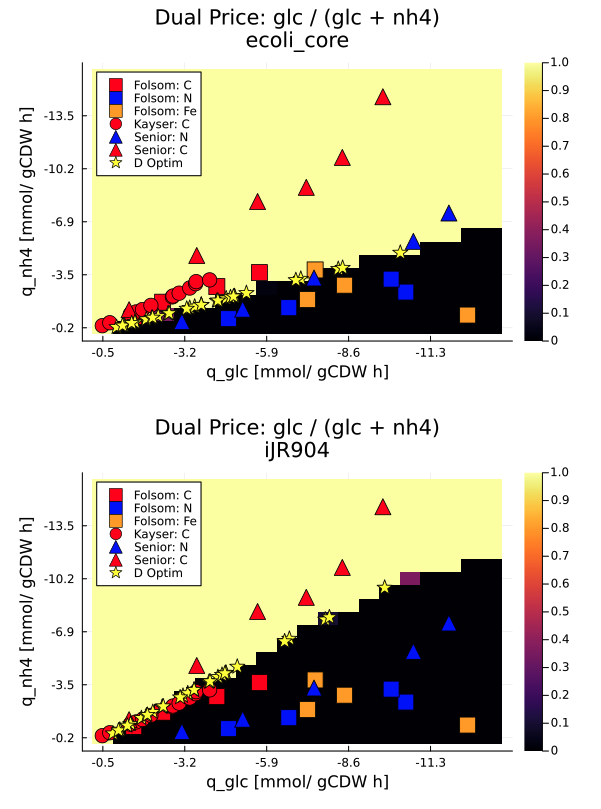
\includegraphics[scale = 0.6]{images/shadow_price_ecoli.png}
% 	\caption{
% 		\textbf{Shadow Prices and Nutrient Limitation for E. coli}:
%         The heatmaps shows the relative value for the shadow price of glucose and ammonia. A number closer to 1.0 indicates that the glucose has must of the join shadow price between the two metabolites for the given flux configuration.
%         The markers are experimental data extracted from the literarure for several nutrient-limited chemostat cultures. 
%         The legend indicates the source and the nature of the limiting nutrient.
%         Additionally, the 'star' markers indicates the optimum usage of the nutrient for the given experimental conditions.
%         The two panels are analogous but uses different metabolic networks, 'ecoli\_core' (72, 95) and 'iJR904' (761, 1075). 
% 	}
% 	\label{fig:shadow_price_ecoli}
% \end{figure}

% \begin{figure}
% 	\centering
% 	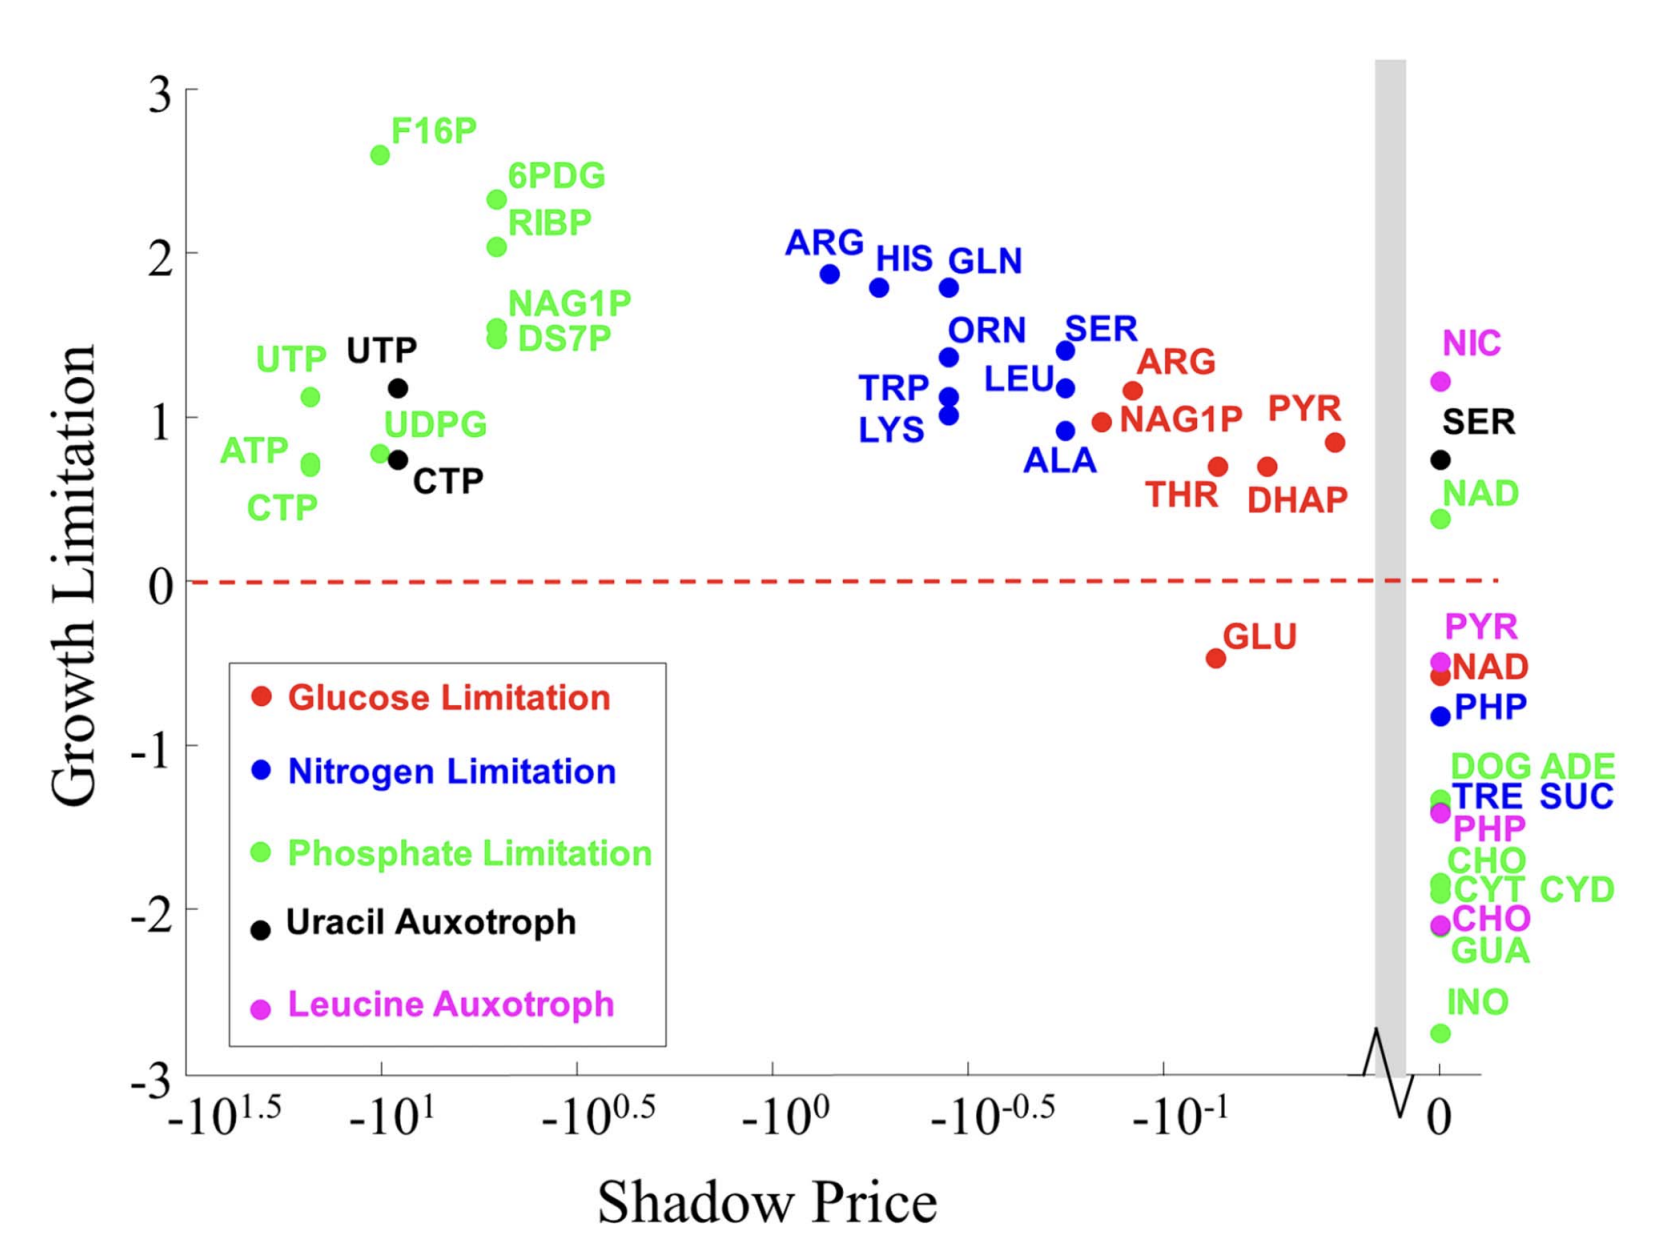
\includegraphics[scale = 0.5]{images/shadow_price_yeast.png}
% 	\caption{
% 		\textbf{Shadow Prices and Nutrient Limitation for Yeast}:
%         (TODO: HERE WE WILL MAKE OUR OWN ANALYSIS/FIGURE EQUIVALENT WITH THE E. COLI (FIGURE \ref{fig:shadow_price_ecoli}). I'LL WILL INCLUDE MORE DATA POINTS). See main text for discussion. The y-axis is an experimental measure of metabolite limitation (possitive $\Rightarrow$ limiting, negative $\Rightarrow$ non-limiting).
% 		The x-axis is the theoretical shadow price.
% 		Taked without permission from \cite{reznikFluxImbalanceAnalysis2013}. 
% 	}
% 	\label{fig:shadow_price_yeast}
% \end{figure}

% We can test how well our definition of nutrient limitation fit experimental data.
% We collected external flux data for E. coli chemostat cultures from the literature [cite required]. The results are presented in Figure \ref{fig:shadow_price_ecoli}, which compares two networks: the widely-used E. coli core network (95 reactions, 72 metabolites) [cite required] and a genome-scaled network iJR904 (761 reactions, 1075 metabolites) [cite required].

% The figure displays a matrix (as a heatmap) that shows the relative shadow prices of two nutrients, glucose and ammonia, as a function of their exchange values. 
% The objective function used is the biomass equation. 
% Specifically, we calculated the change in the upper bound of the biomass reaction as a result of perturbations in the nutrients around a particular exchange setup.
% The colors of the heatmap are arranged such that yellow areas indicate a non-zero shadow price for glucose, while the ammonia price is negligible. 
% Thus, glucose should be the limiting nutrient in these areas.
% Conversely, black areas indicate that ammonia should be the limiting nutrient instead.

% The experimental data from several E. coli chemostat cultures under different nutrient limitation conditions is presented on top of the heatmap.
% The markers are placed at the cultures coordinates (intake of ammonium, intake of glucose).
% With good accuracy, the shadow price predicts the condition of the given culture.
% Specifically, red markers from carbon-limited cultures fall inside (or close to) the yellow area, while blue markers from nitrogen-limited cultures fall inside (or close to) the black area.
% These results suggest that E. coli is growing close enough to the limit allowed by the limiting nutrient intake such that this flux becomes one of the effective constraints of the system.

% Aditionally, the same pattern is observed in Yeast chemostat cultures for simple media with different limiting cutrients. Figure \ref{fig:shadow_price_yeast} show the results of a similar analysis carried by \cite{reznikFluxImbalanceAnalysis2013}. The the y-axis show the experimentally measured dependency of the growth rate ($\mu$) and a given metabolite concentration ($M$), express as $\log(M)/\log(\mu)$. Note that in this work the analysis is extended to internal metabolites as well. In the x-axis they computed the shadow price for each metabolite. The results shows a large majority of metabiolites identified as limiting ($\log(M)/\log(\mu) > 0$) displaying a non zero shadow price. On the other hand, the non limiting metabolites $\log(M)/\log(\mu) < 0$ presented, in large, a zero shadow price. (TODO: HERE WE WILL MAKE OUR OWN ANALYSIS EQUIVALENT WITH THE E. COLI. I'LL WILL INCLUDE MORE DATA POINTS)


% Extending this heuristic to other conditions or more complex organisms is not entirely clear.
% First, it assumes that the maximum possible biomass output is the relevant phenotype to measure.
% Additionally, it relies on the assumption that external constraints, such as given intake fluxes, are part of the effective constraints that describe the system.
% However, there is evidence that mammalian cells use essential nutrients with high efficiency [cire required].
% Furthermore, this procedure is highly dependent on the specific definition of biomass used.

% \subsection{Nutrient-limited network 'cloud'}

% (NOTE: JUST ME TALKING, NO GRAMMAR, NOTHING)

% \begin{figure}
% 	\centering
% 	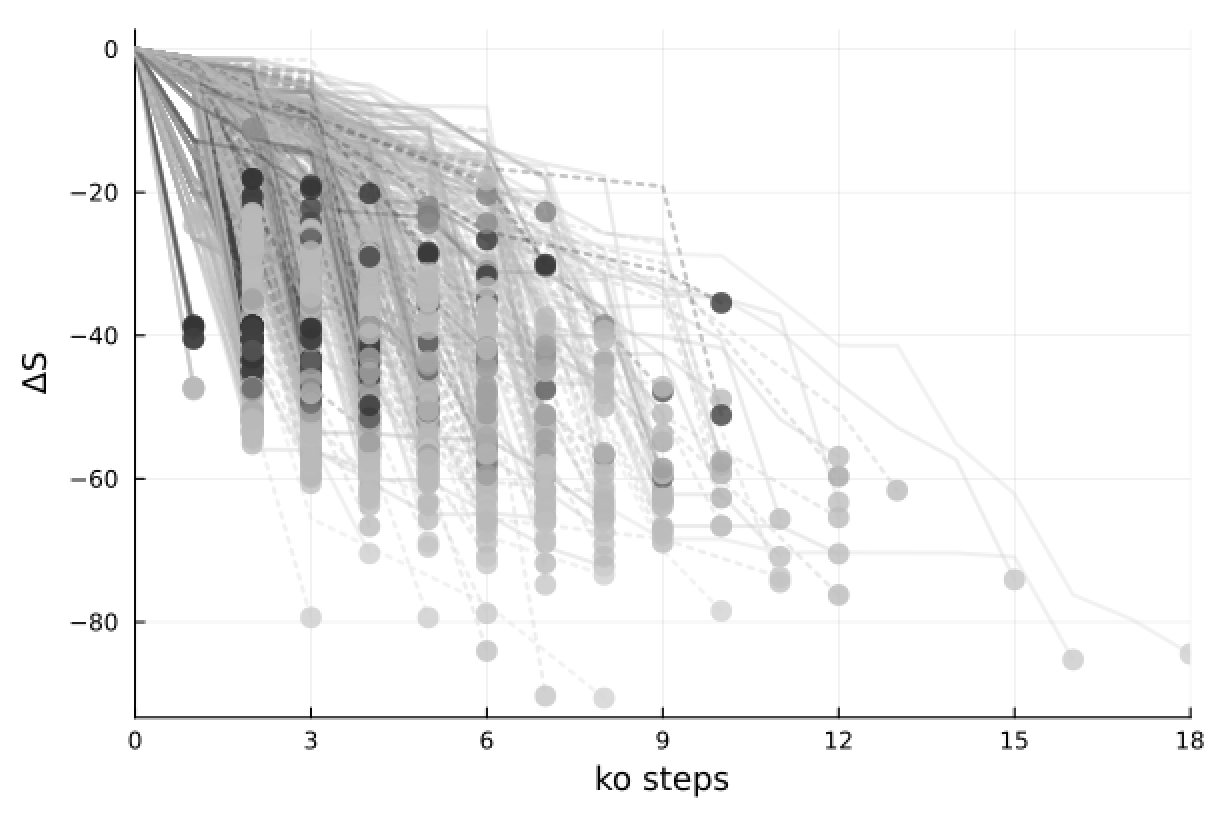
\includegraphics[scale = 0.6]{images/mod_traj_hek.png}
% 	\caption{
% 		\textbf{Informational trajectories of nutrinet-limited subnetwoks for HEK}:
%         Each line is the information of the HEK network as it is modified.
%         At the end (circle), it is glucose limited as desired.
% 	}
% 	\label{fig:mod_traj_hek}
% \end{figure}

% Figures \ref{fig:mod_traj_hek} shows the results (as an illustrative example) of the full methodology employ using a HEK network that is made glucose-limited.
% Basically we just have a cloud of nutrient-limited networks that we can explore. 

% \subsubsection{Theoretical analysis}

% We can performance difference theoretical analysis/integration of the information contained in the network 'cloud'.
% One branch it is just topological studies. For instance, study the frequency of reaction deletions, both at reaction and subsystem levels, and try to find a general pattern. We can of course, do further clustering of the cloud data using the biomass reduction, the entropy reduction, etc. In my opinion, for this to be valuable, we should use high quality networks. We have access to state of the art E coli, Yeast, CHO and Human1. The (used) HEK network is not a good example. 

% The second branch of purely theoretical analysis is the integration of all individual networks into a common model. We can relax the homogeneity constraint and say that the cells can display any of the phenotipes describes by any of the networks in the 'cloud'. One way of persuing that is integrating analitically all the MaxEnt-EP distribution of individual networks into a join model (see Figure \ref{fig:EP_marginals_HEK}). 

% A related idea is to define a probability/weight for each network base in some heuristic. It can be the biomass reduction, the entropy reduction, or the minimal number of blocked reaction required to makes it. We can discusess a minimal action principle: The networks which needs less regulation intervention (eg. less ko reactions) is the more plausible. 

% We can also explore 'clouds' for different nutrients (eg: the 'cloud' for each aminoacid). It might be that a given nutrient can't be limiting (empty 'cloud').


% \begin{figure}
% 	\centering
% 	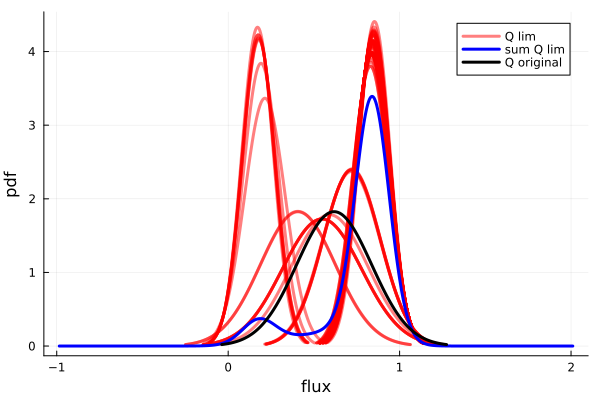
\includegraphics[scale = 0.5]{images/EP_marginals_HEK.png}
% 	\caption{
% 		\textbf{MaxEnt-EP distributions}:
%         Marginal distributions for a particular HEK internal flux.
% 		$Q~original$ is the distribution of the non processed network.
% 		$Q~lim$ are the distributions of 100 nutrient limited subnetworks.
% 		$sum~Q~lim$ is just the normalized addition of all $Q~lim$  (here all networks are equally relevant).
% 	}
% 	\label{fig:EP_marginals_HEK}
% \end{figure}


% \subsubsection{Experimental validation}

% Of course a homerun is to find some kind of experimental validation/analysis relating the 'cloud' networks with data from nutrinet-limited cultures.
% Here we have ZERO results. The closest are the possitive cases for simple mediums (Figures \ref{fig:shadow_price_ecoli} and \ref{fig:shadow_price_yeast}). But there, the 'cloud' does not exist because the initial network already reproduce the nutrinet-limiting phenotype. 
% We need to find studies focused on nutrient limited cultures with complex medium.
% Any mammalian culture will due, but I have more hope to find Yeast/EColi studies.
% Till now we have zero mammalian culture, and all Yeast and EColi but with simple medium.
% This is the current issue stoping us.


% % Experimentally, we have almost nothing about complex media cultures, which mustly involve mammalian cells.
% % This is one stoping point right now.
% % For E coli and yeast I have found a good number of stodies focusing on nutrinet limitation, but all using simple medium.
% % For simple medium we just can't generate a cloud of nutrient-limited network because the original often already are.
% % The perfect situation is to find studies of Yeast/Ecoli focusing on nutrinet limitation but on complex medium.
% % Specificaly transcriptomic and/ir metabolomics, just like \cite{reznikFluxImbalanceAnalysis2013}.




% % \begin{figure}
% % 	\centering
% % 	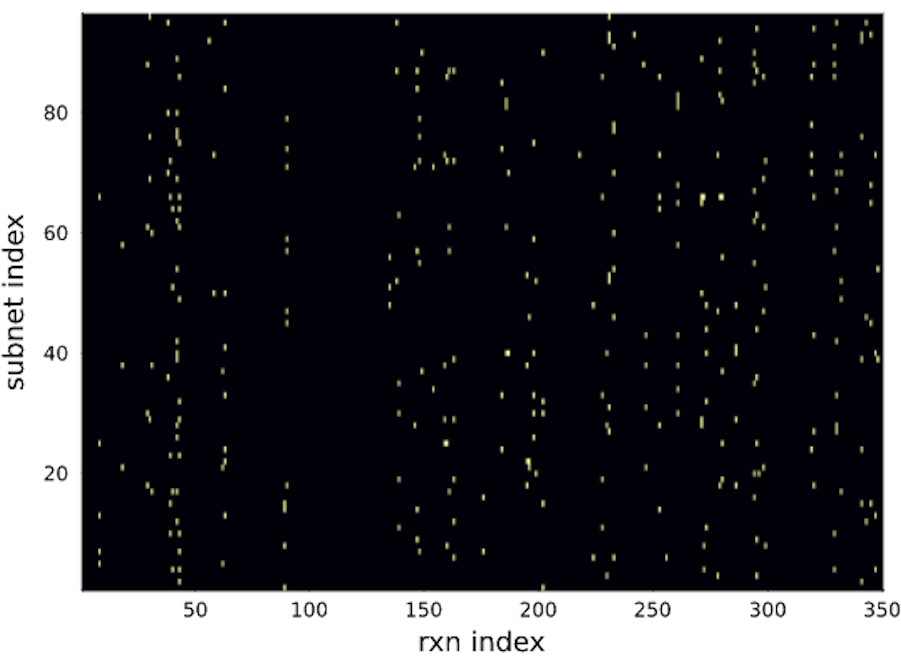
\includegraphics[scale = 0.4]{images/frec_mat_hek.png}
% % 	\caption{
% % 		\textbf{KO aligment of the subnetworks for HEK}:
% %         Each bright spot signal that the given reactions (column) was KO in the given modified subnetwork (row).
% % 	}
% % 	\label{fig:frec_mat_hek}
% % \end{figure}





% % -------------------------------------------------------------------------
% \section{Material and Methods}

% We use Julia \cite{bezansonJuliaFreshApproach2017}

% \bibliographystyle{plain}
% \bibliography{2023_NutrientLimiting_paper}



















% % \begin{figure}
% % 	\centering
% % 	\includegraphics[scale = 0.105]{images/figure_6}
% % 	\caption{ Caption in the next page. }	
% % 	\label{fig:toy_corrs}
% % \end{figure}
% % \addtocounter{figure}{-1}
% % \begin{figure} [t!]
% %   \caption{
% % 	Correlations between the dynamic (x-axis) and inferred mean values (y-axis) for the free fluxes $\zcell$, $\ugcell$ and $\uocell$ of the toy network.
% % 	Each row shows the results of one inference method and each column of one free flux.
% % 	In the case of the $\FBA$ formulations, we specify the sequence of objective functions required to determine a solution
% % 	by using a character triple where: 'm' means minimization, 'M' maximization, 'f' that the flux was fixed to a given value and '0'
% % 	that no further action was required.
% % 	The position of the character express the action over $\zcell$, $\ugcell$ or $\uocell$ respectively
% % 	(Ex: 'M00' means that the maximization of $\zcell$ lead to a single solution).
% % 	The size of the markers encode the value of $\epsilon \in [0.001,1]$.  
% %   }
% % \end{figure}

	
\end{document}
